\section{Discussion} \label{sec:discussion}


\begin{itemize}

    \item

        Discuss that we would have liked to train an RNN on the character limit
        but that we did not have the computation power.

    \item

        Discuss how comparable our results will be with data in the real world.
        We had no texts written by actual ghost writers so we have no idea how
        our networks would perform on such texts.

    \item

        Discuss how different weight functions performed compared to other
        weight functions and describe why we think that is the case.

    \item

        Generate AUROC curves for our networks and discuss the output.

    \item

        Discuss that we beat our baselines but were not able to beat the MaCom's
        restrictions.

\end{itemize}

Looking at the results presented in \ref{sec:results}, is apparent that we've
hit at several points of the spectrum. While none of our methods did achieve
the sub 10\% accusation error on the test set, that MaCom required, we believe
that some of the methods does in fact show promise within the \gls{NLP} field.
While all the networks we applied to the data beat our initially computed
baselines, best performing network that we've tested, is without a doubt the
\ref{conv-char-NN} neural network. This network had an accusation error closest
to to the one required, in addition to having the highest overall accuracy
in all the categories we tested it on. While this network was in fact the
best, it was closely followed by network \ref{conv-word-char-NN}, while the
\gls{RNN} we also tested had sub-par performance, lending credence to the
applicability of \gls{CNN}s to \gls{NLP} problems. It is however worth noting
that this could very well be due to the infeasibility of running any of our
\gls{RNN}s on the character level of the texts supplied to it. Looking at the
performance of the two \gls{CNN}s, it becomes obvious that the character level
is of great importance when it comes to determining the author of a text. The
sentence level is simply to high of a level when it comes to \gls{RNN}s. We
hypothesize that applying it to a lower level, such as the word level would
greatly increase its performance, as \gls{RNN}s would be able learn based on
the words' relation to one another, and open the door to a more grammar based
learning approach. Looking at \gls{conv-char-NN}, and \gls{conv-word-char-NN},
it would seem that focusing on the word level of the texts seem to actually
hurt the model a bit. We are a bit uncertain as to the reason for this, we do
however have some theories. The reason might be likened with the problem the
\gls{RNN}, \ref{rec-sent-NN} had. The level might actually be a bit to high
for our convolutional networks, the image-equivalent of having a to large
convolutional window, thus ignoring all the small details that are needed
in order to properly determine the author. This also highlight a potential
reason behind the differing performance of networks \ref{conv-char-NN} and
\ref{conv-word-char-NN}. \ref{conv-char-NN} looked had a lot of different size
filter on the character level of the text, whereas \ref{conv-word-char-NN}
traded out some of those character level filter with some filter on the word
level. This might very well have led to \ref{conv-word-char-NN} to missing some
relevant person-specific traits on the character level, such as typos, dots,
commas and the like. It wouldn't even be able to find such traits on the word
level, as the usage of a pre-trained embedding layer means that only correctly
spelled word were even considered.

Another \gls{NLP} advantage \gls{CNN}s has in this context, is the fact that
we are able to more accurately determine what part of the text contributed to
final classification.

\subsection{Teacher Feedback}

In our introduction we reported that we wanted to look at what kind of feedback
we could give to teachers in conjunction with the bare predictions. As explained
earlier the system is not meant to be the final judge of which students are
cheating but are rather meant as a support system for teachers that are
already suspicious. We have looked at what kind of feedback we could give to
teachers. We have focused on the \gls{conv-char-NN} network since it performed
best on the test dataset. We have previously looked at the output of the
feature extraction layer to obtain information on what a specific network
were looking at. We wanted to do something similar for teacher feedback.
Recall that \gls{conv-char-NN} started with a convolutional layer followed
by a max pool layer. We therefore know that the larger the output of the
convolutional layer the more important that particular character sequence
is. The output of the feature extraction can be thought of as in Figure
\ref{fig:feature_extraction_output_example}. Each filter gives a single
output that is the maximum output in any filter position. The combining function
for the third network was the absolute difference. That means that when we
are comparing $t$ and $t'$. That means that the output of the combination
will be high for a particular filter iff the maximum output of that filter is
significantly different for $t$ and $t'$.

\begin{figure}
    \centering
    \textbf{Teacher Feedback Script Example}\par\medskip
    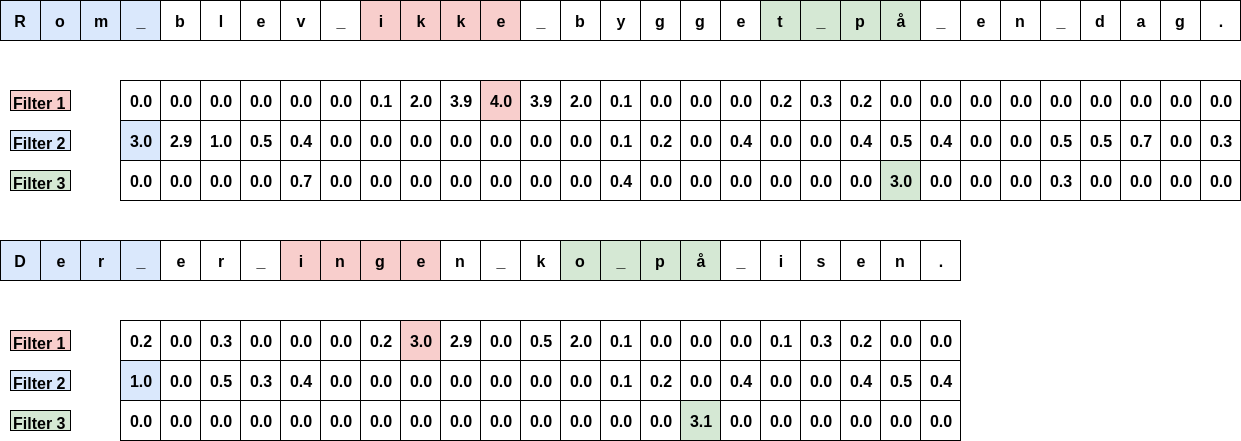
\includegraphics[width=\textwidth]{./pictures/discussion/teacher_feedback_example.png}
    \caption{Illustrates our script that gives feedback to teachers. The
        particular network used in this example only has three filters. The
        three filters maximum activations are shown in three different colors
        for the two texts they are comparing. The first filter looks for
        negative qualifiers. Therefore it reacts strongly to both the Danish
        word "ikke" (not) and the Danish word "ngen" (noone). The second filter
        looks for city names so it reacts strongly to the string "Rom " (Rome)
        but less strongly to "Der " (not a city name) even though it looks like
        a city name. The third filter reacts to phrases that contains the word
        "p\aa " (on) and therefore reacts about the same to both texts.}
    \label{fig:feature_extraction_output_example}
\end{figure}

It is hard to know exactly what the following layers does with the absolute
difference but we feel that it is a fair assumption that the largest filter
differences translates to the most important differences. The feedback system
we implemented for teachers takes an author $\alpha$, text $t$ and $n \in
\mathbb{N}^+$ and outputs the $n$ largest differences between each $t' \in
T_\alpha$ and $t$. The idea is that the when our system reports a negative the
teacher can ask for feedback from the system. The teacher will then get a list
of the $n$ greatest differences between each of the texts and can use that
information to argue against the student.

As an example we ran our system on a random author and a text that that author
did not write. The whole output of three different texts can be seen in Appendix
\ref{subsec:teacher_feedback_text_comparisons} through \ref{TODO}. We have shown
a truncated output in Table \ref{tab:teacher_feedback_output}.

\begin{table}
    \begin{tabular}{llll}
        \textbf{Filter} & \textbf{Activation Text 1} &
        \textbf{Activation Text 2} & \textbf{Difference} \\
        \hline
        426 & \verb'"; ”Hvis "'  & \verb'". Et kla"' & $|2.82 - 4.57| = 1.75$ \\
        71  & \verb'"dem; Nia"'  & \verb'"der skri"' & $|4.64 - 3.16| = 1.45$ \\
        549 & \verb'". Jeg vi"'  & \verb'". Her is"' & $|2.61 - 4.02| = 1.41$ \\
        288 & \verb'" 2 af 2\n"' & \verb'"og refle"' & $|4.90 - 3.53| = 1.37$ \\
        496 & \verb'" udseend"'  & \verb'"vad litt"' & $|2.78 - 4.12| = 1.34$ \\
        33  & \verb'"et sind."'  & \verb'"risning,"' & $|3.05 - 4.36| = 1.31$ \\
        460 & \verb'" 2 af 2\n"' & \verb'" krig og"' & $|3.69 - 2.43| = 1.26$ \\
        514 & \verb'", derfor"'  & \verb'", i forb"' & $|3.82 - 5.06| = 1.24$ \\
        531 & \verb'" om, for"'  & \verb'" om, hva"' & $|4.64 - 5.84| = 1.20$ \\
        458 & \verb'"Derudove"'  & \verb'"derfor b"' & $|4.31 - 3.13| = 1.18$ \\
        \\
        261 & \verb'".\n\n\n"'   & \verb'"– de"'     & $|1.72 - 2.70| = 0.98$ \\
        484 & \verb'"lv; "'      & \verb'" dét"'     & $|2.02 - 2.96| = 0.94$ \\
        17  & \verb'"st ”"'      & \verb'"gt; "'     & $|2.57 - 3.45| = 0.88$ \\
        145 & \verb'"ndet"'      & \verb'" Det"'     & $|2.37 - 3.25| = 0.88$ \\
        299 & \verb'"osse"'      & \verb'"– de"'     & $|3.12 - 3.98| = 0.86$ \\
        477 & \verb'"f 2\n"'     & \verb'"v og"'     & $|3.05 - 2.20| = 0.85$ \\
        421 & \verb'" 13."'      & \verb'" vel"'     & $|3.03 - 2.19| = 0.84$ \\
        434 & \verb'"am; "'      & \verb'" dét"'     & $|1.18 - 2.00| = 0.82$ \\
        27  & \verb'"n to"'      & \verb'"Dett"'     & $|2.20 - 2.99| = 0.79$ \\
        445 & \verb'" om,"'      & \verb'" – S"'     & $|2.51 - 3.27| = 0.76$ \\
    \end{tabular}
    \caption{Shows the 10 most different activations of convolutional filters on
        two different texts. Both the 10 most different activations for the
        filter of size 8 and size 4 is shown. The strings that produced the
        activation are shown and the actual activations are shown to the right.}
    \label{tab:teacher_feedback_output}
\end{table}

We also looked at whether or not we could say something about which parts of an
assignment are the most likely to be ghost written. That would allow a teacher
that is suspicious of a student to identify the part of the assignment that were
least likely to be written by him and look closely at that. To do that we wrote
a script that splits a text into paragraphs and use \gls{conv-char-NN} to get a
score for each paragraph. We can then report which of the paragraphs of the text
are the most likely to be ghost written. To test our script we chose an author
$\alpha$ from the validation dataset C with $|T_\alpha| = 19$. We also chose a
random text $t \in \overline{T_\alpha}$. We took out one of the texts $t' \in
T_\alpha$ and let $T = T_\alpha \setminus \{t'\}$. We then combined $t$ and $t'$
into $t''$ such that $t''$ consist of all of the text $t'$ followed by a random
paragraph from the text $t$. That is we constructed a text $t''$ that consisted
of a text in $T_\alpha$ followed by a single paragraph not from $T_\alpha$. We
then used our script to predict which part of $t''$ was most likely written by
a ghost writer. We would expect that the last paragraph in $t''$ would be the
most likely. The output of the script was a vector of the probability of each
paragraph having been written by a ghost writer.

\begin{equation}
    (0.66320, 0.60432, 0.54737, 0.47438, 0.30528)^T
\end{equation}

As expected the last paragraph is the least similar and therefore most likely to
be written by someone else. We are now able to give a teacher an idea of why our
network makes the predictions it does. We can give feedback on which parts of
the text is the least characteristic of an authors writing style and we can give
feedback on why the network thinks that. Of course a teacher will still have to
make the ultimate decision but can use the output of the network to underpin his
or her accusation.


\subsection{Applicability of Method}

In this section we will discuss how applicable our approach will be to real
world situations. We have created our solutions in a lab setting which
simplifies the problem quite a bit. We discuss here how our results can be
applied to find real ghost writers.

The biggest problem with our approach is that we had no actual ghost written
assignments available. We were given a dataset of authors where each author had
written a set of assignments. To create ghost written assignments we used
assignments turned in by other authors. It would of course have been better if
we had had a dataset of authors where each author had a set of assignments known
to be written by him/her and a set of assignments known to have been written by
a ghost writer hired by that author. That was not possible however since MaCom
did not have that data. In a real ghost writer setting the ghost writer might
try to mimic the writing style of a student and in that way might trick our
algorithm into classifying a \gls{FP}.

We have discussed another problem with our dataset during the experiments we
performed. We observed multiple times that the network were reacting strongly
to strings looking like Danish names and school class identifiers. On our
artificially constructed dataset all of an authors texts will have the correct
name and most generated ghost written texts will have a different name.
Therefore names are an excellent feature to look at due to the way our dataset
was constructed. In a real ghost writer setting however the names attached to an
assignment is a useless feature as a ghost writer will always put the students
name on the assignment. We have tried to work against these deficiencies of our
dataset by removing as many names as possible and as much other information as
possible.

We know that we removed a significant amount of information from the texts since
we observed the training and validation accuracy falling after the change. We
also saw less of the filters looking at text metadata suggesting that it is not
as important to the networks.

It is hard to predict exactly how well the network will perform on ghost written
assignments when we had no such assignments available during testing. However we
believe we have handled the deficiencies in the dataset as well as possible.


\subsection{Weight Functions}

As described in Section \ref{subsec:prediction_system} we use several weight
functions to weight which of an authors texts are most important. Looking
at the graphs in Section \ref{subsubsec:prediction_system_conv-char-NN},
\ref{subsubsec:prediction_system_rec-sent-NN} and
\ref{subsubsec:prediction_system_conv-char-word-NN} we can get an idea of the
relative strengths of the weight methods. Using those graphs we want to discuss
a couple of the weight functions.

\begin{description}

    \item[$P_\mathrm{U}$]

        The uniform weight function generally has a lower accuracy and higher
        accusation error than the other weight functions. The only weight
        function that performs worse than the uniform weight is the $P_{min}$
        weight function. We had expected that the uniform weighing would perform
        worse than the other since it doesn't use any metadata about the texts
        to make its predictions. It only use the raw predictions on the texts of
        the networks and simply takes an average of that.

    \item[$P_{exp_\lambda}$]

        The exponential dropoff weight function used the time of an assignment
        to determine the most important text. Recall that as $\lambda
        \rightarrow \infty$ more weight is placed on the newest assignment. We
        assumed that an authors writing style would change over time and the
        newest text would therefore be a better predictor of current writing
        style than the oldest text. Since all time based weight functions
        performed better than uniform weights our assumption must have been
        correct.

        When looking at the performance over the different $\gamma$ values we
        tried, we observed that the accuracy tends to increase at the extremes
        of the graphs as $\gamma$ increases while it falls around the peak of
        the graphs as $\gamma$ increases. The accusation error tends to be
        highest in the beginning for high $\gamma$'s and lowest in the end for
        high $\gamma$'s.

        The accusation error at the end of the $\theta$ spectrum is irrelevant
        for this assignment as the accusation error is too high for all weight
        functions at that point. However it is very important that the
        accusation error is low in the beginning. As we lower $\gamma$ nearing a
        uniform weight we get a lower accusation error in the beginning of the
        graph at the cost of some accuracy.

        \begin{figure}
            \centering
            \textbf{TITLE}\par\medskip
            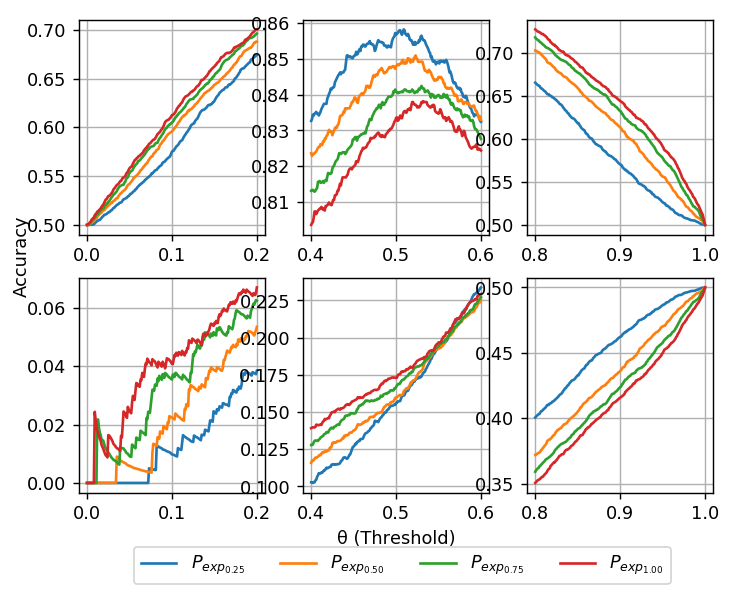
\includegraphics[width=0.7\textwidth]{./pictures/discussion/conv_char_nn_prediction_zoom.png}
            \caption{Illustrate important intervals for our different
            $P_{exp_\lambda}$ prediction systems. On the left we have shown the
            beginning of the curves, in the middle we have shown the top
            accuracy and to the right we have shown the end of the curves.}
            \label{fig:conv_char_prediction_zoom}
        \end{figure}

\end{description}
